% Part: biographies 
% Chapter: alonzo-church 
% Section: biography
\documentclass[../../../inclu
de/open-logic-section]{subfiles}

\begin{document}

\olfileid{bio}{alc}{bio} 
\olsection{Biography}

\begin{figure}[h!]
 \centering
 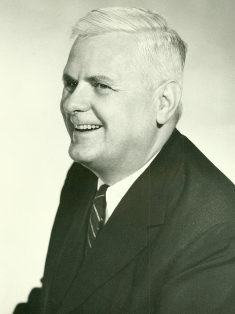
\includegraphics[scale=0.8]{alonzo-church.jpg}
\caption{Alonzo Church. Photo Credit: Wikimedia.} 
\end{figure} 
Alonzo Church was born in Washington, DC on June 14, 1903. He is perhaps
 best known for the Church-Turing thesis and Church's theorem, although he
 publushed also in set theory and philosophy.
 
 In esaly childhood, an air gun incident left Church blind in one eye 
 \citep[2]{Enderton2016}. He finished prepratory school in Connecticut in 1920 
 and began his univeristy education at Princeton that same year. He completed his
 doctoral studies in 1927. After a couple years abroad, Church began his
academic career back at Princeton. Throughout his career he was known as
a polite and careful man. His blackboard writing was immaculate, and he would
carefully preserve important papers by carefully covering them in Duco cement
\citep[4]{Enderton2016}. Outside of his academic pursuits, he enjoyed reading
science fiction magazines and was not afraid to write to the editors if he
spotted any inaccuracies in the writing \citep[5]{Enderton2016}.

Church's achievments were great. He developed a theory of
effective calculability, the $\lambda$ calculus, independently of Alan
Turing's development of the Turing machine. The two definitions of
computabiliy are equivalent, and give rise to what is now known as the
\emph{Church-Turing Thesis}, that a function of the natural numbers is
effectively computable if and only if it is computable via Turing machine.
He also develped what is now known as \emph{Church's Theorem}: The 
decision problem for the validity of first-order formulas is unsolvable.

Church continuted his work into old age. In 1967 he left Princeton for UCLA
 in order to pursue his work with the \emph{Journal of Symbolic
Logic}. He was professor there until his retirement in 1990. Church passed
away on August 1, 1995 at the age of 92.


\end{document}